\documentclass[11pt]{report}
\usepackage{fancyhdr}
\usepackage{fancybox}
\usepackage{tipa}
\usepackage{framed}
\usepackage[retainorgcmds]{IEEEtrantools}
\usepackage[utf8x]{inputenc}
\usepackage{epsfig}
\usepackage{anysize}
\usepackage{gensymb}
\usepackage{amssymb}
\usepackage{graphicx}
%\usepackage[demo]{graphicx}
\usepackage{caption}
\usepackage{subcaption}
\usepackage[utf8x]{inputenc}
\usepackage{longtable}
\usepackage{url}
\usepackage{plain}
\renewcommand{\bibname}{References}
%\usepackage{hyperref}
\usepackage[plainpages=false]{hyperref}
\hypersetup{
    colorlinks=true,
    linkcolor=black,
    citecolor=black,
    filecolor=black,
    urlcolor=black,
}
\lhead{}


\setcounter{page}{-100}
\setcounter{secnumdepth}{5}

\newenvironment{fminipage}%
{\begin{Sbox}\begin{minipage}}%
{\end{minipage}\end{Sbox}\fbox{\TheSbox}}
% Title Page
\title{\textbf{Analyzing Security Specification Of Android O.S On DALVIK V.M}}
\vspace{2.5cm}
\author{\bf{A Seminar Report}\\
        \\
        \emph{Submitted in partial fulfillment of requirements for the degree of}\\
        \\
        \bf{Master of Technology}\\
        \\
        \emph{by}\\
        \\
		\bf{Mohit Singh}\\
        \bf{Roll No : 143050099}\\
        \\
        \emph{under the guidance of}\\
        \\
        \bf{Prof. R.K. Shyamasundar}\\
        \\\\
        
\includegraphics[height=3.5cm]{./images/iitb_logo}\\
        \\
        \bf{Department of Computer Science and Engineering}\\
        \bf{Indian Institute of Technology, Bombay}\\
}
\date{MAY, 2015}


% page layout settings

% \setlength{\parindent}{2pc}
% \setlength{\oddsidemargin}{50pt}
% \setlength{\evensidemargin}{50pt}
% \setlength{\marginparwidth}{50pt}
% \setlength{\textheight}{9.0in}
% \setlength{\topmargin}{-0.75in}
% \setlength{\footskip}{30pt}

\marginsize{2.5cm}{2.5cm}{1cm}{1.5cm}
\setlength{\headheight}{15pt}

\pagestyle{fancy}

\usepackage{graphicx}
\begin{document}
\maketitle
\pagenumbering{roman}
\tableofcontents
%\listoffigures
%\listoftables
\begin{abstract}
With the development of smart-phone technology, smart-phone(Android) applications are becoming an important part of our daily life. Now a days,
Android applications are being used  extensively for e-commerce \& sensitive operations (like bank transactions), 
which has attracted attention of some bad guys. And due to wide exposure of Android activity/services,
any Android security vulnerability can be exploited by attackers. In this Report,\textbf{"Analyzing Security Specification Of Android O.S On DALVIK V.M"} and we are going to implement some more 
security features in it.
\end{abstract}
%@dollars
\pagenumbering{arabic}




\chapter{Introduction}
\label{chapter:intro}
Android is one of the most popular smart-phone O.S.Now a days we are heavily dependent on our smart-phone that it contains all are information about us starting from  personal pics to bank details.
ALL this make the Android a hot shot for the attackers.taking this matter serious we need to Analyzing Security Specification Of Android O.S and then try to suggest some more enhancement to the existing Android
to make it more secure but without compromising on the flexibility and ease of development.starting with the introspection of Android O.S we need to demonstrate some possible attacker on the existing Android environment.
\section{introduction  to information flow control} 
Now after discovering the vulnerability we want to take few steps in direction of making it more secure and for that we are using the concept of "information flow control"
the motivation behind "information flow control is to guarantee the secure information flow in the computer system"[site danning paper].
In order to carry out further we want to use this beautiful concept in the modern mobile operating system (“ANDROID”).
In short it allows only those application to interact which follows the policies defined by the concept of "information flow control" to make it more secure but still accessible and flexible for the developer to develop an application.



\chapter{ANDROID Architecture}
Before playing with the system it is better to know more about the system.In this section we taking the overview of the system,taking some knowledge about its Architecture ,what are the basic components does it have.

\par
starting with the ANDROID Architecture in which we are focusing only on the application framework part.
  \begin{figure}[ht!]
\centering
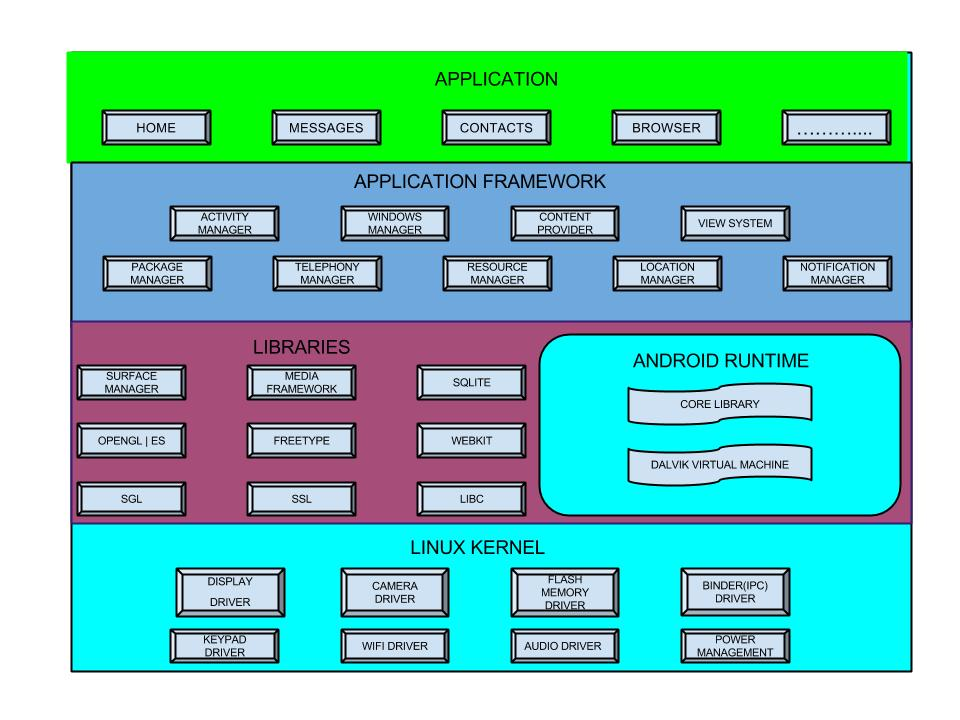
\includegraphics[width=150mm]{./images/system.jpg}
\caption{ Fig shows the Android Architecture. \label{overflow}} \cite{fig}
\end{figure}
Android operating system is a stack of software components which is roughly divided into five sections and four main layers as shown above in the architecture diagram.
\begin{enumerate}
 \item \textbf{Linux kernel:} is to  provides basic system functionality like process management,memory management, device management like camera, keypad, display etc
 \item \textbf{Libraries:}is section in which set of libraries are useful repository for storage and sharing of application data.
 \item \textbf{Android Runtime:}is main component in the whole architecture which is sophisticated Java Virtual machine for Android.this allows multiplication application to run simultaneously in isolation with each other.
 
  \item \textbf{Application Framework:} provides higher-level services to application .this gives developer a privilege to use number of predefined services in their application.
 \item \textbf{application:} is on top at the hierarchy which is solely meant to serve the end-user. 
 \end{enumerate}

\section{Application Fundamentals:}
Java is one of the most powerful and versatile programming languages and may be the reason it is being used to develop the Android Application.ANDROID 
SDK is used to generate the APK file. which is ready to get installed on any mobile any ANDROID machine.
\par
Android run each application in its own sandbox. 
\begin{description}
 \item[$\bullet$]In Android, each application run as a different user having its own set of permission which given by the system at the time of installation of the application.  
 \item[$\bullet$]Each application has its own unique user id (UID) set by the system at the time of installation.
  \item[$\bullet$]"Each process has its own virtual machine (VM), so an app's code runs in isolation from other apps".\cite{fun}
 \item[$\bullet$] An application started when it's component is called at stop when it in not in use.

\end{description}
\par
An application can access its own component only and other application's component directly.
This doesn't mean that two different applications can not interact with each other.their other ways to do this also.
\begin{description}
 \item[$\bullet$] It is possible that two different application can have same user id.By this mean two application can interact with each other.
 In order to save resources the two application share the same user id are used to run the same virtual machine.
 But this can only be possible when the application is signed with the same same developer key.
 
 \item[$\bullet$]The manifest.xml file is the file which contains all the permission request of an applicability.

\end{description}
\subsection{App Components}
As we come to know that there are multiple numbers of components in a single application which means there can be multiple numbers of entry point in our application. 
but not all component can be the entry point to the system.For a component to be an entry point in the application either it defined as exported component or they do have an intent filter for that component in the 
manifest file .
\par
There are four different types of application components.Each one has its own functionality to offer and their lifetime is is the function of their requirement.
\linebreak
Here are the four types of application components:

\begin{description}
 \item[$\ast$Activities:] An activity the is single screen user interface which is mainly used to interact with user,Although they collectively perform operation to make good user experience.
 \par
 For example, a camera app can start new google drive activity to backup the images. 
 \item[$\ast$Services:]A service is a component which mainly used to do long time taking background process.Example the process of downloading a file is an example of long time taking a process 
 which can be run in the background.Generally services are not intended to have any interface to interact with the user.

 \item[$\ast$Content providers:]A content provider handles the set of applications data.Suppose store the contact is stored in the (persistent storage  location ) which can be queried  by any application 
  with the proper set of permission and hence that query is handled by the Content provider.Content providers can also be used to manipulate the data that is private to that application which is making the request.


 \item[$\ast$Broadcast receivers] "A Broadcast receiver is a component that responds to system-wide notifications".\cite{fun}
 Example: while using the camera if the battery goes down then the system will broadcast an announcement and in respond to that the broadcast handler of the camera will close the camera application.
\end{description}
\section{Permission Model}
Android is based on Linux's kernel but in spite of that its permission model is different in quiet different my many aspect.In Android each process/application is treated as a different user having a set of permission that 
can only be assigned by the system at the point of installation.Each application run in a basic sandbox which isolates application from each other and provide the basic functionality.
When the application wants to access some permission protected system level API then it has to request it from the system explicitly by mentioning the permission in the manifest.
the View of Manifest.Xml file is shown to the user that these are the set of permissions this application wants and after knowing that you still wants to install this application.
\subsection{Requesting Permissions}
It is advised to not to take permission which has no use and try to minimize the set of permission as much you can. Because this minimizes the risk of having security threat to the application, as well as to the system.
\par
four types of protection level.
\begin{description}
 \item[$\bullet$ "Normal permission] are granted automatically by the system .pre-configured in Sandbox."\cite{analyZING}
 \item[$\bullet$"Dangerous Permission]can only granted at the time of installation by the user.If the user is not allowed those permissions then the application is not installed."\cite{analyZING}'
 \item[$\bullet$"Signature permission]can only granted by if the requesting application is signed by the same developer that defend the permission. 
 signature permissions are useful to restrict  component access to a small set of application trusted and controlled by the developer  "\cite{analyZING}
\end{description}
In the above section, we saw that how an application can gain capabilities by asking for permissions.We know that the “great power comes with great responsibility”.An application can gain
“ dangerous permission” only at the time of installation. After that the application can do whatever it wants to do with those set of permission . 
\textbf{Now what's our point of discussion is that by any means an application is not able exploit the permission that it doesn't have.}
\par
In addition to the permission, we also have to handle the permission protected API carefully because there may be a chance that the malicious application 
can invoke your activity and request to get done some suspicious thing which require you permission to carried it out. It advised to not to leak the permission protected data to any application that request it,
because that data you are going to generate require some special permission that is assigned to you at the time of installation and the requested application doesn't have those permission.
\par
 we have to restrict all those  inter-application communication through which they can harm the user. Without reducing the functionality of our system.
 In this report we are going to discuss the Android application interaction and identify security risks in the application components.\par


\section{Intents}
Android provides the bells and whistles to make development of android applications easier than before.
INTENT which is the message passing system of android is one of a kind.With the help of INTENT we can link different components of an application .
It allows application to interact with each other,it supports both inter-application as well as intra-application communication.\\
Intent can be categories in two type
\subsection{Types Of Intent}
\begin{description}
 \item[$\bullet$Explicit intent] is the form of INTENT which takes the components name (the fully-qualified class name ) as an input from developer of the application to start that component.
 the intended use of explicit intent is for intra-application communication because only developer should know the name and path its component.
\par
 Intent downloadIntent = new Intent(this, DownloadService.class);
 \par
 downloadIntent.setData(Uri.parse(fileUrl));
\par
startService(downloadIntent);
  \begin{figure}[ht!]
\centering
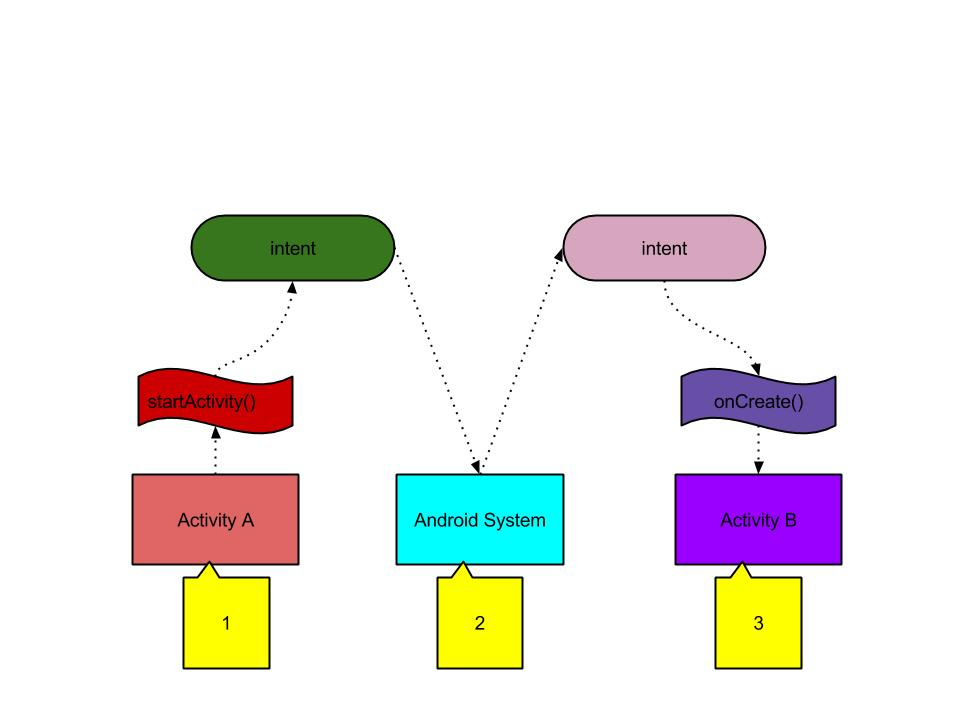
\includegraphics[width=90mm]{./images/impin.jpg}
\caption{ Fig shows the ANDROID architecture. \label{overflow}}
\end{figure}
 \item[$\bullet$Implicit intent]"In Implicit intent is not named a specific component, But instead declare a general action to perform, which allows a component from another application to handle it. For example,
 if we want to show the user a location on a map,we can use an implicit intent to request that another capable app show a specified location on a map."\cite{if}
 
 \end{description}

\par 
\textbf{we are concentrating of the vulnerability related to implicit INTENT only}  

\chapter{Security In Android}

"Android comes with the security features built in it seems to be promising when it comes to reducing the frequency of impact significantly.
it comes with some default permission like system and file in order to reduce the Critical decisions about security"\cite{st}

\subsection{Core Security Features That Used to Build Secure Application:}
\begin{itemize}
  \item Each application run in Sandbox which isolates it with other running application
  
  \item The sandbox run each application with some predefined system level permission, But if application wants to use some permission protected API then it should ask for it explicitly at the time of 
  installation because those permissions protected API (resources) are scheduled by the system which will be shared with other application.
  
  \item "An application framework for robust implementations of common security functionality such as cryptography, permissions, and secure IPC (inter-process communication).\cite{st}"
  \item Android use encrypted file system in order  to protect the data, from theft, loss 
  
  \item User grants the ''dangerous permission``  to the application on files or restricted access at the time of installation.
  
  \item "Application-defined permissions to control application data on a per-app basis".\cite{st}
  
  \item "An application can specify that the caller must have  a certain permission by adding the permission requirement to a component declaration in the manifest or setting a default permission 
   The requirement for whole application.\cite{analyZING}
  
  \item "The developer can add permission check throughout the code. Conversely, a broadcast intent by Requiring the recipient to have  a permission.
  (this protection is only to broadcast intent and not available to activity or service intents) "\cite{analyZING}

\end{itemize}
 
for the later chapter all the above are the prerequisite concept.
in the later chapter we will get to know ho these components are actually interact with each other and how many attacker are their. 
\chapter{system design}

before dealing with that attacker scenario on the system and the proposing the solution for that first we have to define our system
\section{ system configuration}
Here is the configuration details of our system which we are using for all our practice related to this project.
  \begin{figure}[ht!]
\centering
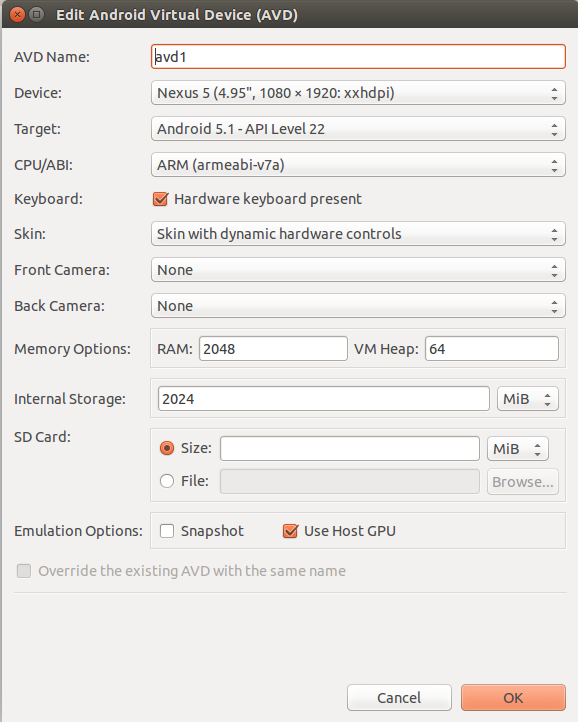
\includegraphics[width=90mm]{./images/spec.png}
\caption{ Fig shows the Specification of our system. \label{overflow}}
\end{figure}
apart from all are technical specification we are dealing with.the most significant one is the Target android version that we are 
dealing with.It is clearly visible that we are using the latest android version 5.1 (Lollipop) having API level=22.
which is the latest till the date of experiment.this shows that we are working with the cutting edge specification and any vulnerability
to this system may have some serious consequences in the near future.


\section{Attack Scenario}
\subsection{ Internal Activity Invocation Or Confused Deputy,}
Suppose you have an application which is miss-configured in a way that the application uses implicit intent for internal communication.
We have to define an intent filter to capture the incoming intent.But due to this Although we have not defined it as a exported component the
component becomes accessible from the outside of this application.Due to this fact any malicious application can demand for 
some unethical functionality from that component or can get infected data.The receiver component will still 
thinks that this INTENT is from trusted source (send by some component from the same application) then due to this assumption it will not go for any verification of the INTENT.
which make the application vulnerable.as a result of this either it can return some sensitive data to the malicious calling class which compromises the permission protected information,
In this case their is no need of any permission to the caller, or corrupted its own sensitive file by writing the infected data to the file.

\begin{figure}
\centering
\begin{subfigure}{.5\textwidth}
  \centering
  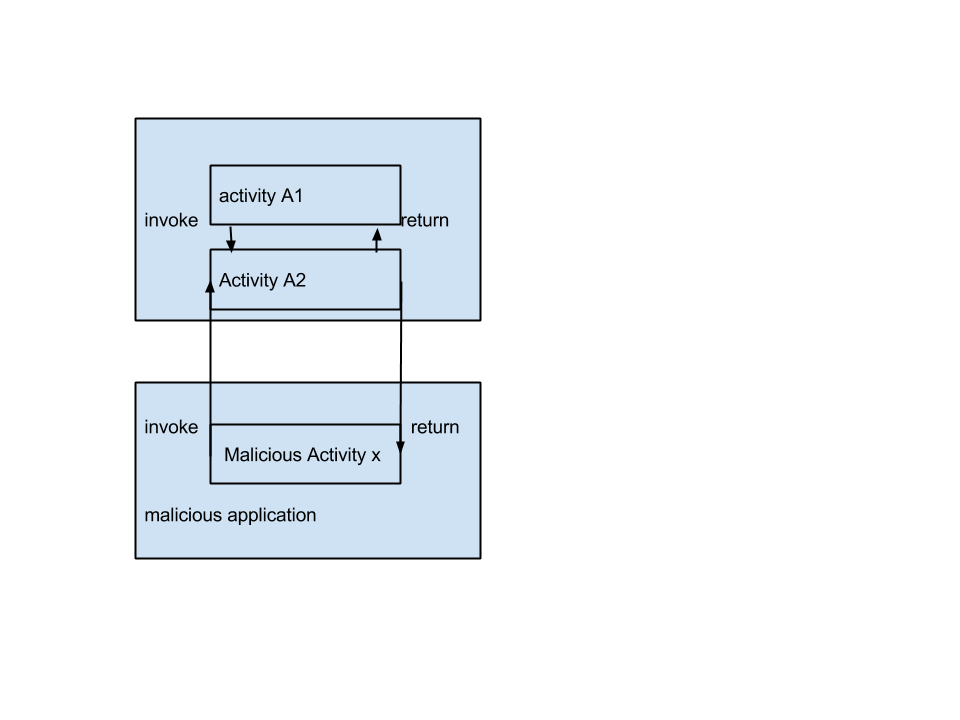
\includegraphics[width=1\linewidth]{./images/a1.png}
  \caption{internal Activity invocation or confused deputy}
  \label{fig:sub1}
\end{subfigure}%
\begin{subfigure}{.5\textwidth}
  \centering
  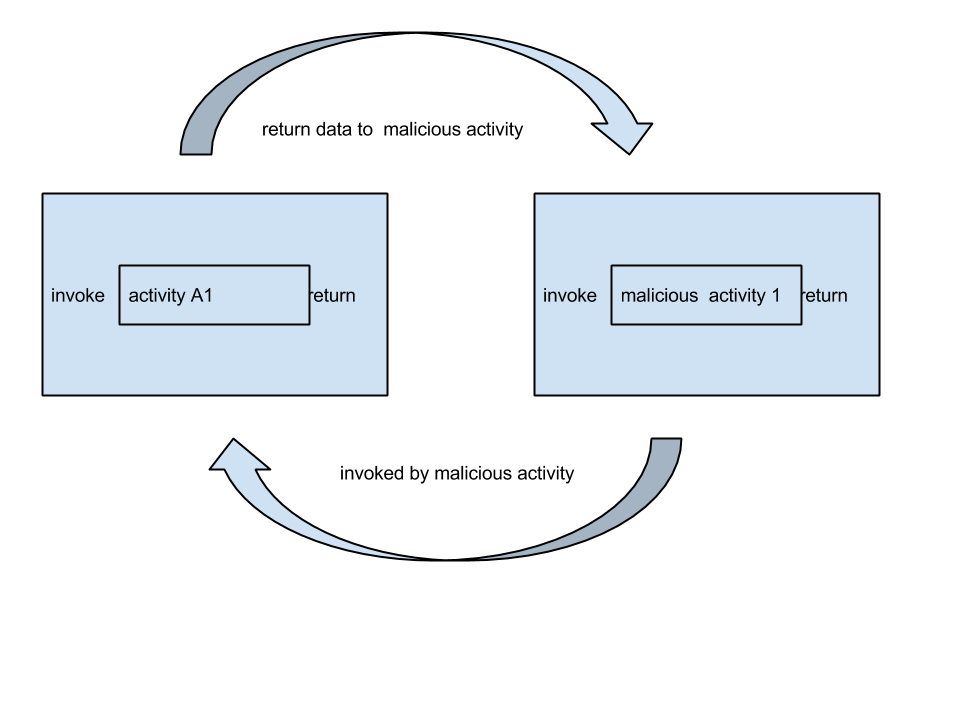
\includegraphics[width=1\linewidth]{./images/a2.png}
  \caption{application sharing user ID with a compromised application}
  \label{fig:sub2}
\end{subfigure}
\caption{A figure with two subfigures}
\label{fig:test}
\end{figure}




\subsection{Application Sharing User ID With A Compromised Application}
In this Attack the malicious application tricked the victim application
by saying that the caller application sharing use id with the victim application
and asking for the permission protected information. In spite of the fact that in victim's 
application's components is able to handle unknown application request.But it is failed to check 
the permission of the callee.



\subsection{Collusion Attacks}
In this type of attack two malicious application can collectively produce the leakage of 
sensitive or Permission protected information from flow .and in this type of attack their is nothing can be done because in this case both sender and receiver
are corrupted .So the concept like check the callee before returning the data will not work here.
this type of attack can only tackled if and only if the Android O.S will check the authenticity of both the application.

\section{Rules That Should Be Followed.}
\begin{enumerate}
\item Use explicit intent while sending private or confidential data .

\item use explicit intent for intra-application communication.

\item while using implicit intent make sure that the intent should be permission protected.

\item You should do the verification of the source of intent while the returning some data on completion of its call.

\item Make sure that, those components that are not intended to interact with  other application should not be exported. 

\item you should be aware of that ,while declaring the intent filter for a component you are making that component accessible
to other application also .even when you haven't declared as the exported component.

\item those action which are able to change state of an application should not be declared in the exported component.

\item make two different component to serve the intent .one for inter-application and other one for intra-application

\item In the exported component make sure that the intent is form valid source before taking any action.
 
\item "Intent filters are not security measures and can be bypassed with explicit Intents. Requiring Signature or SignatureOrSystem permissions is an effective
way of limiting a component's exposure to a set of trusted applications. their analysis reveals that developers commonly use the action field of an Intent like
an address instead of explicitly addressing the Intent."\cite{analyZING}

\item component accessibility should be divided into three categories: internal, exported to the system only, and exported to
other applications.\cite{analyZING}

\end{enumerate}


\chapter{Information Flow Control}
with the help of this mechanism we can formulate the mathematical framework for classify the secure information flow
 between the different level of security classes.the mathematical framework is based on the lattice.
 In our system neither any lower class application ask for information from higher class application nor any higher class application is able to 
to send information to lower level  However class higher class application can ask for information from lower class application and lower 
level class application can send information to higher level class.
In order to enforce the information flow control in android their are number of challenges that we have to face.\\
\section{Defining the System}
But first we have to define our system .\\
\textbf{Subject} in our case are the applications \\
\textbf{Object} in our case are the implicit intent \\
as we have seen in the previous chapter that the security class of an subject is defined by the set of reader and writer permission.
In the previous section we have discussed that how an application gain permission.
now we have to categories the android permissions in two different set 
\textbf{READ PERMISSION} and another one is \textbf{WRITE PERMISSION}.
on the basis of read and write permission assigned to application at the time of installation we can classify the class of application each and 
every application.
\[\textrm{hence when an application }A_1\textrm{ has set of read permission }R_1\textrm{ and set of write permission }W_1\]
\[\textrm{ send an implicit intent }I_1\textrm{ then the intent will have the following signature 
}(A_1,R_1,W_1)\]
\section{Defining policies for interprocess communication}
After defining the rules of information flow control in the previous chapter now we have to formulate those rules in the form of system policies.
On the basis of these system policies the Android should be able to take decisions which set of application can interact with each other.
and which set application are not allowed to talk.
\subsection{interaction between application}
under what condition application are allow to interact.
this can be explained with the help of example.
\[\textrm{suppose in our system we do have to an application} A\textrm{ having set of read permission }R_A \]
\[\textrm{ and set of write permission }W_A  \]
and their are number of application which can handle intent sent by A on the basis of its action.form that set of application we have to chose 
from those application which follows ours information flow control policies.
and this can we done by comparing the set of read and write permission of sender application with receiver application.
then we can define the set of application that \[\textrm{can handle the intent send from application } A_1 \textrm{ be X } \]
\[\forall x_i \in \textrm{\{set of installed applicaiton\}} \]
then\[ R_{x_i}\textrm{ be the set of read permission of application }x_i\]
and\[ W_{x_i}\textrm{ be the set of write permission of application }x_i\]
\[ if( R_A \supseteq R_{x_i} \textrm{ and } W_A \subseteq W_{x_i})\]
then \[x_i \in X\]
else \[x_i \notin X\]

\section{Implement Of Information Flow Control}
Now in order to implement the concept of information control we need to make a monitor which is nothing other that an application itself.
But Monitor is not like an ordinary application it is a kind of system application which does have some super user level permission.
\par 
the basic functionality of Monitor is to perform a validation check  on the incoming implicit intent.and then suggest which application is 
safe to chose as the receivers of that implicit intent.
\par
but the question is where we have to place our monitor ? being a system application we don't have many choice regarding the positioning of 
our application hence we have to make our system application as a universal receiver which is able to handle each and every type of intent.
after getting the intent we will do multiple number of operation  and then suggest the possible receiver application for this intent.after that 
we have to resent the intent to the system and this time on the basis of our suggestion. we have to pick the right application.
\section{Categorize System Level Permission}
In our system we do have total 209 permission.on the basis of its permission's description we have to manually separate these permission in two set 
READ Permission set and other one is write permission set.
so at the end we do have a hash map  at our monitor of the all the 209 permissions which are mapped to a set S having only three elements in it and the
set S= {READ,WRITE,READ/WRITE}.
  \begin{figure}[ht!]
\centering
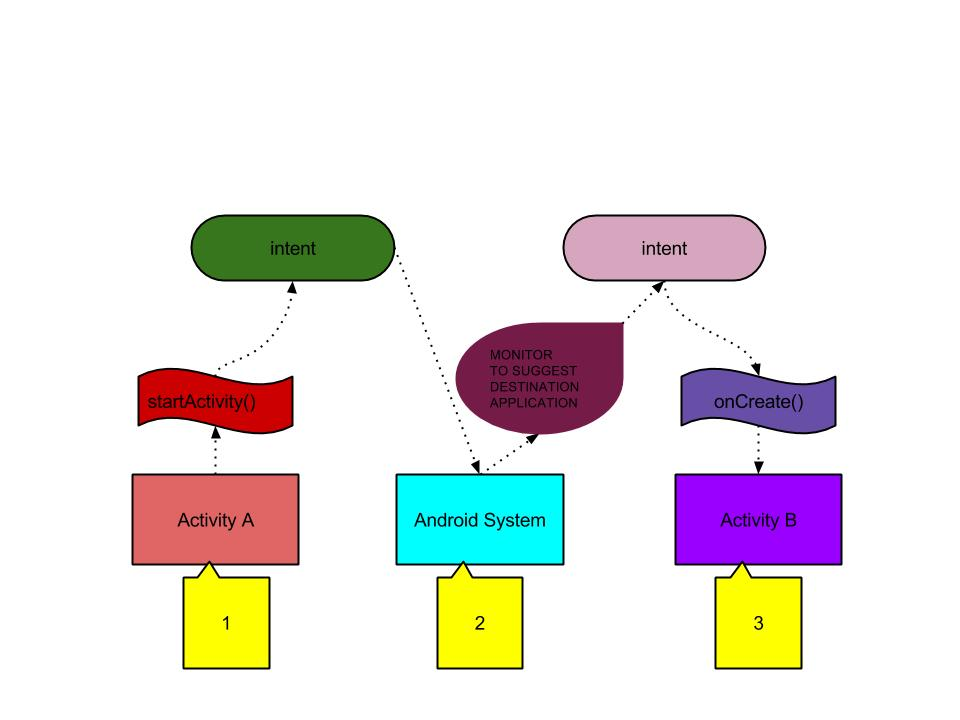
\includegraphics[width=150mm]{./images/monitor.jpg}
\caption{ Fig shows the Specification of our system. \label{overflow}}
\end{figure}

\section{Monitor Intercept All Implicit Intent}
for the effectiveness of our monitor it is necessary that each and every implicit INTENT should be pass through our monitor.that is in the manifest file of 
our monitor we have to make INTENT filter corresponding to the component which is doing the validation check.the use to INTENT-filter is that it will project the component in front of 
android system that it can handle each and every type of implicit intent.
\section{Operation On Intent}
After the successful intercept of intent 
we need two basic information from that intent 
\begin{enumerate}
 \item source application/package of intent. 
 \item on the basis of action define in the intent what are the possible receiver application/package of that intent.
 
\end{enumerate}
\par 
but we do have a small issue here and that is not all implicit intent carry their source application name.
and without the knowledge of source application it is nearly impossible to implement the information flow control.
So we taking the assumption that all INTENT does have its source application name in it.

\section{Operation For Finding Correct Receiver Application}
once we got the source application/package and list of all possible application that can handle this intent.
we need to get all the PERMISSION corresponding to source application and  all possible application that can handle this intent.
after that we have to compare the permission of the source application with the hash map which is define in the above section.
on the basis of hash map we  have to separate list of permission in two set read set and write set corresponding to each application.
if 

\[ \textrm{in this case A be the source of intent. } R_A \textrm{ be the set of read permission of A }\]
\[ W_A \textrm{ be the set of write permission of A }\]
\[\forall x_i \in \textrm{\{set of all applicaiton that can handle this intent \}} \]
then\[ R_{x_i}\textrm{ be the set of read permission of application }x_i\]
and\[ W_{x_i}\textrm{ be the set of write permission of application }x_i\]
\[ if( R_A \supseteq R_{x_i} \textrm{ and } W_A \subseteq W_{x_i})\]
then \[x_i \in X\]
else \[x_i \notin X\]

hence we will suggest only those application that are in set X.because they are the safest choice 
among all the application

\chapter{Conclusion}
\label{chapter:conclusionandfuturework}
android is a good mobile operating system.In order to provide the extensive support of ease of development it is somewhere lacking behind on the security front.
that makes it vulnerable and become the easy Target for hacker.in the result of implementations of information flow Control we have found that most of unsecured information flow 
can be restricted but we have to pay the cost because their are many false positive result due to which many application are not allowed to interact with each other.
\section{Future Work}
till now we dealing with only implicit Intent .but interaction between two different application can also done via explicit intent. 
and we are unable to intercept the explicit intent.but if we want to make Android totally secure we need to implement information flow control in the code of android itself.
with take huge amount of time and resources.

\begin{thebibliography}{100} % 100 is a random guess of the total number of
%references
\addtolength{\leftmargin}{0.2in} % sets up alignment with the following line.
\setlength{\itemindent}{-0.2in}
\bibitem{denning}  Denning, D. E. (1976). A lattice model of secure information flow. Communications of the ACM, 19(5), 236-243. 
\bibitem{auto} Sbîrlea, D., Burke, M. G., Guarnieri, S., Pistoia, M., \& Sarkar, V. (2013). Automatic detection of inter-application permission leaks in Android applications. IBM Journal of Research and Development, 57(6), 10-1.
\bibitem{analyZING}Chin, E., Felt, A. P., Greenwood, K., \& Wagner, D. (2011, June). Analyzing inter-application communication in Android. In Proceedings of the 9th international conference on Mobile systems, applications, and services (pp. 239-252). ACM..
\bibitem{Book}Robling Denning, D. E. (1982). Cryptography and data security. Addison-Wesley Longman Publishing Co., Inc..
\bibitem{notused} Bartsch, S., Berger, B., Bunke, M., \& Sohr, K. (2013, September). The Transitivity-of-Trust Problem in Android Application Interaction. In Availability, Reliability and Security (ARES), 2013 Eighth International Conference on (pp. 291-296). IEEE.
\bibitem{notused2} Grace, M. C., Zhou, Y., Wang, Z., \& Jiang, X. (2012, February). Systematic Detection of Capability Leaks in Stock Android Smartphones. In NDSS.
\bibitem{st} \url{http://developer.android.com/training/articles/security-tips.html}
\bibitem{if} \url{http://developer.android.com/guide/components/intents-filters.html}
\bibitem{fun}\url{site http://developer.android.com/guide/components/fundamentals.html}
\bibitem{fig}\url{http://www.tutorialspoint.com/android/android_architecture.htm}

\end{thebibliography}
\end{document}